\chapter{Diseño de la variante \emph{DC-Net}}

\section{Glosario de Términos}

\begin{itemize}
    \item Participante: agente que participa activamente del protocolo, ya sea 
    enviando un mensaje o contribuyendo para aumentar el tamaño del 
    \emph{anonimity-set} y así ocultar ``de mejor manera'' a los emisores de 
    mensajes. 
    \item Ronda: serie de pasos (descritos a partir de la próxima sección) que 
    se llevan a cabo (principalmente intercambiando mensajes entre los 
    participantes) con el objetivo de ir reduciendo ronda a ronda los mensajes 
    enviados por cada participante.  
    \item Mensaje: información que cada participante desea transmitir de 
    manera anónima. Generalmente se relacionará a un conjunto de caracteres 
    (representados como \emph{String}), en un cierto idioma, que se desea 
    enviar.
    \item Sesión: conjunto de rondas que se necesitan realizar para que pueda 
    ser transmitido, a lo más, un mensaje por participante. Al principio de 
    cada sesión, se le da la oportunidad a cada participante de decidir si 
    enviará o no un mensaje. Luego que cada participante realizó su decisión, 
    se inicia el protocolo descrito a continuación, que tiene como objetivo 
    que cada uno de los mensajes que se decidieron enviar, se envíen de manera 
    anónima al resto de los participantes.
    \item Sala: conjunto de participantes corriendo una sesión del protocolo.
    \item Observador Externo: cualquier agente (a excepción de los propios 
    participantes) que pueda estar monitoreando, tanto los mensajes 
    resultantes del protocolo, como mensajes intermedios intercambiados entre 
    los distintos participantes durante la realización del protocolo. A no ser 
    que se explicite, todos los mensajes del protocolo pueden ser monitoreados 
    por un observador externo.
    \item Adversario: agente que tiene como finalidad, ya sea encontrar al 
    emisor de un cierto mensaje, o bien, alterar el comportamiento ``normal'' 
    del protocolo (retrasándolo o impidiendo su total realización). Este 
    adversario puede ser un mismo participante del protocolo (al cual 
    llamaremos participante malicioso) o un observador externo.
\end{itemize}

\section{Diseño a primera vista}

El protocolo propuesto tiene como principal característica el no evitar las 
posibles colisiones que puedan producirse (idea que se distancia de otros protocolos 
que se enfocan en evitar la colisión de mensajes). De producirse la colisión, se 
debe resolver corriendo nuevas rondas del protocolo, pero solamente permitiendo 
que un subconjunto de los mensajes colisionados puedan re-enviarse en cada una 
de las rondas subsecuentes, produciendo así que en cada ronda nueva que se 
desarrolle, exista un menor número de mensajes colisionando, resultando así 
en rondas que se desarrollen sin colisión, enviándose los mensajes de manera 
solitaria, lo que les permite ser legibles por el resto de los participantes.

\todo{agregar diagrama de resolución de colisiones}

\section{Compartición de Llaves}

Una ronda real comienza con el proceso de compartición de llaves entre cada 
par de participantes presentes en la sala. Este proceso debe realizarse, 
tomando un cuenta un posible adversario que esté monitoreando el canal de 
comunicación existente entre dos participantes cualquiera.

Para solucionar este problema se propone el uso del algoritmo 
\emph{Diffie-Hellman} \cite{diffie1976new} que permite generar un valor 
secreto compartido entre dos agentes, cuyo canal de comunicación es 
monitoreado por un adversario.

Luego que cada par de participantes $\{P_i, P_j\}$ ejecuten el algoritmo 
\emph{Diffie-Hellman}, obtendrán un valor secreto $k_{ij}$. Para futuros pasos 
del protocolo, es necesario que ejecuten este proceso dos veces, ya que es 
necesario que cuenten con un segundo valor compartido $r^k_{ij}$.

\subsection{\emph{Commitments} sobre las llaves}

Posteriormente cada participante $P_i$ debe realizar un \emph{commitment} a 
cada valor $k_{ij}$ que posee compartido con cada otro participante $P_j$, 
utilizando como aleatoriedad el segundo valor compartido, $r^k_{ij}$. Esto 
resulta en que cada participante posee $n - 1$ de los siguientes valores 
$c_{k_{ij}} = g^{k_{ij}} h^{r^k_{ij}}$.

Luego de esto, cada participante $P_i$ generará dos valores, el primero será 
la suma de todas las llaves compartidas que posee $K_i = \sum k_{ij}$. El 
segundo valor será un \emph{commitment} sobre dicho valor, esto es, 
$c_{K_i} = \prod c_{k_{ij}}$.

Finalmente cada participante $P_i$ enviará al resto de la sala vía 
\emph{broadcast} su \emph{commitment} $c_{K_i}$ junto con una 
\emph{zero-knowledge proof} demostrando que conoce los valores ``escondidos'' 
dentro del \emph{commitment}.

\subsection{Verificación de los valores enviados}

\todoline{Verificar zkp, multiplicacion de commitments de llaves y como encontrar al culpable}

\section{Formato del Mensaje}

Al principio de una sesión, cada participante $P_i$ debe decidir si desea comunicar un mensaje $msg$ al resto de la sala o no. De querer enviar un mensaje, habrán rondas que deberá enviar $m_i = msg$, y otras que enviará $m_i = 0$. De no querer transmitir un mensaje, en todas las rondas enviará $m_i = 0$. 

Para que el protocolo funcione correctamente, es necesario que dicho mensaje $m_i$ se concatene con otros valores, permitiendo el correcto manejo de colisiones de mensajes (es explicado más adelante en el documento). Estos valores auxiliares son los siguientes:
\begin{itemize}
    \item $b_i$: bit que indica si el participante esta, en la presente ronda, enviando un mensaje distinto a cero o no ($b_i = 1 \iff m_i \neq 0$).
    \item $pad_i$: cadena de bits aleatoria que se añade para prevenir colisión de mensajes iguales, que podría desembocar en que la sesión nunca finalice.
\end{itemize}

Con estos valores establecidos, en cada ronda cada participante $P_i$ debe formar el siguiente valor $M_i$:

\begin{figure}
  \centering
    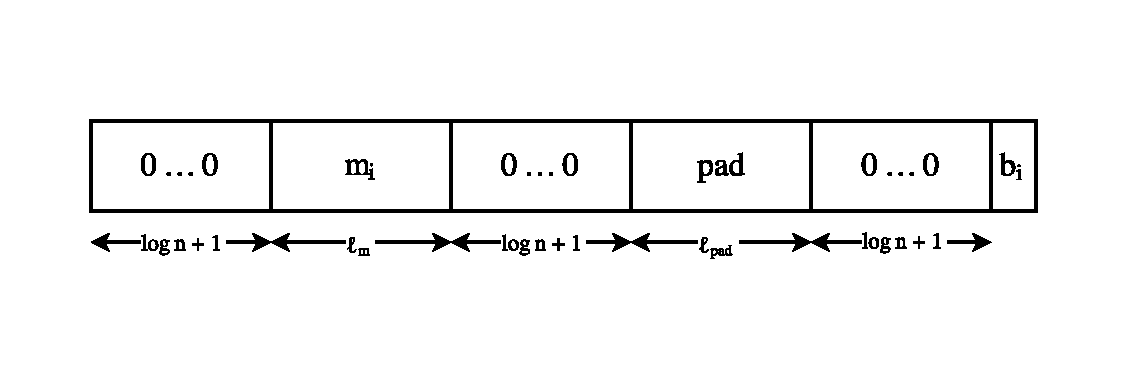
\includegraphics[width=1\textwidth]{imagenes/message-format(1).pdf}
  \caption{$M_i$ cuando se envía un mensaje}
\end{figure}

\begin{figure}
  \centering
    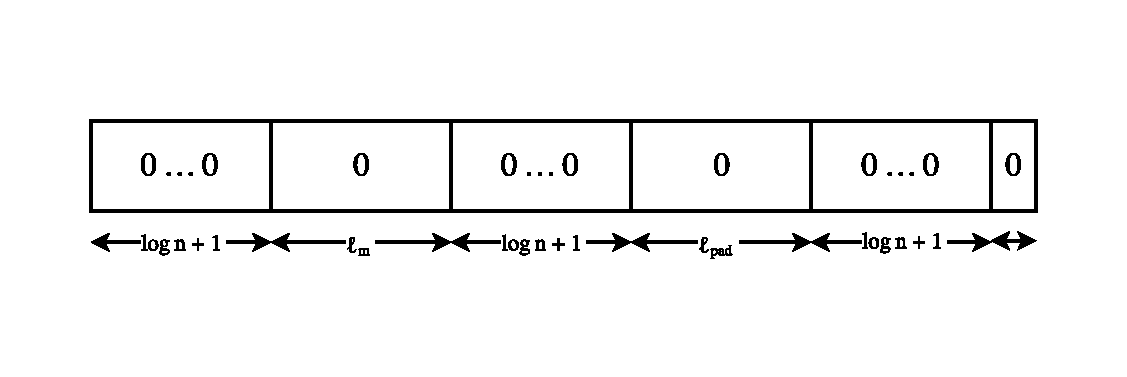
\includegraphics[width=1\textwidth]{imagenes/message-format-nomessage.pdf}
  \caption{$M_i$ cuando no se envía un mensaje}
\end{figure}

\section{Correctitud del Formato del Mensaje}

Para que el protocolo tenga un correcto funcionamiento en el manejo de colisiones, es imperioso que el formato del mensaje $M_i$ se respete por todos los participantes. Para ello se debe satisfacer una de las siguientes restricciones:
\begin{itemize}
    \item Si $b_i = 0$, entonces $m_i = 0$
    \item $b_i = 1$
\end{itemize}
En la primera alternativa, se le fuerza al participante a que si esta diciendo que no envía un mensaje ($b_i = 0$), no lo envíe ($m_i = 0$). En la segunda opción, se le permite cualquier valor de $m_i$ siempre y cuando se cumpla que $b_i = 1$.

\subsection{\emph{Commitments} sobre los valores individuales}

Para poder demostrar que su mensaje $M_i$ posee un correcto formato, es necesario primero realizar \emph{commitments} a cada uno de los valores $\{m_i, pad_i, b_i\}$. Para ello, se escogen valores aleatorios $\{r_i^m, r_i^{pad}, r_i^b\}$ y se calculan los valores $c_{m_i} = g^{m_i} h^{r_i^m}; c_{pad_i} = g^{pad_i} h^{r_i^{pad}}; c_{b_i} = g^{b_i} h^{r_i^b}$ (\emph{commitments} a los valores individuales anteriormente descritos).

\subsection{\emph{Zero-knowledge Proof} sobre formato del mensaje}

Ahora es momento que cada participante genere una \emph{zero-knowledge proof} que demuestre que el mensaje $M_i$ esta bien formado. Para ello es necesario establecer primero si en la presente ronda el participante enviará un mensaje ($m_i \neq 0$) o no ($m_i = 0$).

\begin{enumerate}
    \item No envío de mensaje ($m_i = 0$): para demostrar que el formato es correcto cuando no necesito enviar un mensaje, cada participante debe demostrar la primera restricción que se mostró anteriormente, esto es, que $b_i = 0 \land m_i = 0$.
    
    Es importante notar que cuando sucede lo anterior, los valores de los \emph{commitments} anteriormente descritos quedan de la siguiente manera: $c_{m_i} = h^{r_i^m}; c_{b_i} = h^{r_i^b}$.
    
    Finalmente lo que el participante debe demostrar es que conoce los valores $\{r_i^m, r_i^b\}$ contenidos en dichos \emph{commitments}.
    \item Envío de mensaje ($m_i \neq 0$): para demostrar que el formato es correcto cuando necesito enviar un mensaje, debo demostrar la segunda restricción, esto es solamente que $b_i = 1$.
    
    Al igual que en el caso anterior el \emph{commitment} relacionado queda con un formato particular $c_{b_i} = g h^{r_i^b}$.
    
    En este caso se le va a pedir al participante demostrar que conoce $r_i^b$ en $g^{-1} c_{b_i} = h^{r_i^b}$.
\end{enumerate}

Como no se puede saber si el participante enviará o no un mensaje (comprometería su anonimato) se va a solicitar que demuestre cualquiera de las dos condiciones anteriores. La \emph{zero-knowledge proof} que necesita demostrar cada participante es la siguiente: $$\mathtt{PoK_i^{format}} = PoK\{(r_i^m, r_i^b) : (c_{m_i} = h^{r_i^m} \land c_{b_i} = h^{r_i^b}) \lor (g^{-1} c_{b_i} = h^{r_i^b})\}$$

\subsection{Envío de valores a la sala}

Después de todos los cálculos anteriores, cada participante $P_i$ debe enviar al resto de la sala vía \emph{broadcast} los siguientes valores: $\{c_{m_i}, c_{pad_i}, c_{b_i}, \mathtt{PoK_i^{format}}\}$ (los tres \emph{commitments} calculados y la demostración correspondiente).

\subsection{Verificación de la demostración}

Después de que toda la sala haya recibido todos los conjuntos de valores enviados por cada uno de los participantes, es necesario verificar que la demostración sea correcta, y para ello solamente es necesario los valores de los \emph{commitments} acompañando la \emph{zero-knowledge proof}.

\section{Demostración de conocimiento del mensaje}

Cada particiante $P_i$ debe enviar un \emph{commitment} sobre el mensaje $M_i$ construido anteriormente, con el objetivo que más adelante envíe el mensaje que ha estado construyendo durante la presente ronda. Para construir dicho \emph{commitment} utilizará los \emph{commitments} de los valores individuales enviados anteriormente. Para ello calculará $c_{M_i} = f(c_{m_i}, c_{pad_i}, c_{b_i})$\footnote{$f(x, y, z) = x^{2^{|pad|}(n+1)} y^{(n+1)} z$} $= g^{M_i} h^{r_i^{M}}$ (donde $r_i^{M}$ es un valor aleatorio definido por los valores $r_i^m, r_i^{pad}, r_i^b$). 

Luego de esto se necesitará que cada participante envíe una \emph{zero-knowledge proof} demostrando que conoce los valores $M_i, r_i^M$ dentro de $c_{M_i}$: $\mathtt{PoK_i^M} = PoK\{(M_i, r_i^M) : c_{M_i} = g^{M_i} h^{r_i^M}\}$.

\subsection{Verificación de la demostración}

Por cada participante $P_j$ que envía la demostración anterior, es necesario primero formar el valor $c_{M_j}$ utilizando los valores de los \emph{commitments} recibidos anteriormente de la siguiente manera: $c_{M_j} = f(c_{m_j}, c_{pad_j}, c_{b_j})$.

Luego de esto, es posible verificar la demostración $\mathtt{PoK_j^M}$ utilizando el valor $c_{M_j}$ construido anteriormente.

\section{Envío del mensaje de salida}

En este punto, cada participante $P_i$ ha demostrado la correctitud de los valores con que se ha comprometido a enviar (hasta ahora, solo ha enviado \emph{commitments} y demostraciones, ningún valor ``útil'' para la ejecución del protocolo).

Cada participante $P_i$ generará el valor $O_i = K_i + M_i$ (denominado mensaje de salida). Este valor tiene como objetivo ``ocultar'' al mensaje $M_i$ sumándole el valor secreto $K_i$. Informalmente, cuando un participante reciba un mensaje $O_i$, no podrá discernir si este mensaje de salida contiene o no un valor $M_i \neq 0$.

Ahora bien, es necesario realizar una distinción con respecto a lo que cada participante necesita demostrar con respecto a su mensaje de salida $O_i$. Cuando se desarrolla la ronda 1, solo es necesario demostrar que dicho mensaje $O_i$ se forma a través de los valores ``ocultos'' en los \emph{commitments} $\{c_{K_i}, c_{M_i}\}$ enviados anteriormente ($c_{M_i}$ no se envió explícitamente, pero se construyó a partir de los \emph{commitments} individuales que sí se enviaron).

En las rondas posteriores, la demostración se vuelve más compleja, ya que se necesita demostrar que el valor $M_i$ que forma parte del mensaje de salida $O_i$ es, ya sea, igual a 0 (no le corresponde enviar un mensaje en dicha ronda), o bien, es el mismo mensaje que el involucrado en la colisión más próxima (más detalles serán analizados más adelante).

\subsection{Ronda 1}

Cada participante $P_i$ necesita generar el siguiente \emph{commitment} para $O_i$, $c_{O_i} = g^{o_i} h^{r_i^O}$. Para formar este valor se utilizan los \emph{commitments} enviados anteriormente de la siguiente manera: $$c_{O_i} = g^{o_i} h^{r_i^O} = g^{K_i + M_i} h^{r_i^K + r_i^M} = g^{K_i} h^{r_i^K} g^{M_i} h^{r_i^M} = c_{K_i} c_{M_i}$$

Con lo anterior, se le solicita a cada participante que demuestre en una \emph{zero-knowledge proof} que conoce el valor $r_i^O$ (suma de las aleatoriedades utilizadas en los \emph{commitments} para la llave $K_i$ y el mensaje $M_i$) dentro de un \emph{commitment} especial $c_{r_i^O} = h^{r_i^O}$. La \emph{zero-knowledge proof} resulta en $\mathtt{PoK_i^O} = PoK\{r_i^O : c_{r_i^O} = h^{r_i^O}\}$.

Finalmente cada participante enviará el par $\{O_i, \mathtt{PoK_i^O}\}$ al resto de la sala vía \emph{broadcast}.

\subsubsection{Verificación de la demostración}

Cada participante $P_i$ debe verificar la demostración recibida de cada otro participante $P_j$. Para ello, primero deberá calcular el valor $c_j^O$ como la multiplicación de los \emph{commitments} recibidos en pasos anteriores de la siguiente manera: $c_j^O = c_j^K \cdot c_j^M$.

Luego de esto, deberá calcular, utilizando el valor $O_j$ recibido recién, el valor $\beta_j = c_j^O \cdot (g^{O_j})^{-1} = g^{O_j} h^{r_j^O} (g^{O_j})^{-1} = h^{r_j^O}$.

Finalmente se debe verificar la demostración $\mathtt{PoK_j^O}$ utilizando el valor $\beta_j$ calculado anteriormente.

\subsection{Rondas posteriores}

En rondas posteriores a la primera, se debe asegurar que los participantes estén enviando un mensaje válido, el cual solo puede tener dos alternativas: o bien no envía ningún mensaje (ya sea porque su mensaje ya fue recibido por todos los participantes en una ronda sin colisión, o no está habilitado para enviar mensaje en esta ronda), o envía exactamente el mismo mensaje que se envió al principio (no ha cambiado el mensaje que quiere comunicar en rondas posteriores).

Para lograr esto, es necesario hacer una distinción con respecto a la ronda exactamente anterior a la ronda actual. Si la ronda anterior fue una ronda real, se verifica que el mensaje enviado en la ronda actual sea el mismo que el enviado en dicha ronda anterior; pero si la ronda anterior es virtual, no hay ningún mensaje con el que comparar (no se envía ningún mensaje en rondas virtuales). A esta ronda anterior se le denominará \emph{ronda padre}.

\subsubsection{Ronda padre real}

Si actualmente se está desarrollando la ronda $k$, entonces la ronda padre es la ronda $k/2$. Se va a denotar con un superíndice entre paréntesis la ronda en que se envía cada mensaje.

Primero, cada participante $P_i$ necesita calcular el siguiente valor $\alpha_i = {(c_i^m)^{-1}}^\mathtt{[k]} \cdot {(c_i^m)}^\mathtt{[k/2]}$. El valor $\alpha_i$ representa la multiplicación del inverso del \emph{commitment} sobre el mensajes $m_i$ enviado en la ronda actual con el mismo \emph{commitment}, pero enviado en la ronda padre.

Notar que el valor $\alpha_i$ se utilizará exclusivamente cuando el participante deba demostrar que envía un mensaje. La otra situación (no enviar un mensaje) se demostrará, igual que en un paso anterior, mostrando que $b_i= 0 \land m_i = 0$. Cuando sucede la primera alternativa (enviar un mensaje, y que éste sea igual que al enviado en la ronda padre), $\alpha$ toma el siguiente valor:

\begin{flalign*}
    \quad \alpha_i &= {{(g^{m_i} h^{r_i^m})}^{-1}}^{\mathtt{[k]}} \cdot {(g^{m_i} h^{r_i^m})}^{\mathtt{[k/2]}} &\\
        &= \frac{1}{{{(\cancel{g^{m_i}} h^{r_i^m})}^{\mathtt{[k]}}}} \cdot {(\cancel{g^{m_i}} h^{r_i^m})}^{\mathtt{[k/2]}} &\\
        &= {h^{r_i^m}}^{\mathtt{[k/2]}} \cdot \frac{1}{{h^{r_i^m}}^{\mathtt{[k]}}} &\\
        &= {h^{r_i^m}}^{\mathtt{[k/2]}} - {h^{r_i^m}}^{\mathtt{[k]}} &\\
        &= h^{({r_i^m}^{\mathtt{[k/2]}} - {r_i^m}^{\mathtt{[k]}})} &\\
        &= h^{r_i^{m*}}
\end{flalign*}

Con lo anterior, lo que debe demostrar cada participante $P_i$ en este punto es que su mensaje $O_i$ (enviado en la ronda $k$ actual) cumple una de las siguientes alternativas: (1) codifica un mensaje $m_i$ igual al mensaje $m_i$ enviado en la ronda padre (ronda $k/2$), o (2) codifica un mensaje $m_i = 0$, lo cual se traduce en demostrar que $b_i = 0 \land m_i = 0$. Con esto, la \emph{zero-knowledge proof} necesaria es la siguiente: $$\mathtt{PoK_i^{O, real}} = PoK\{(r_i^b, r_i^m, r_i^{m*}) : (c_i^b = h^{r_i^b} \land c_i^m = h^{r_i^m}) \lor (\alpha_i = h^{r_i^{m*}}) \}$$

Luego de calcular la \emph{zero-knowledge proof} anterior, cada participante $P_i$ va a enviar al resto de la sala vía \emph{broadcast} el par $\{O_i, \mathtt{PoK_i^{O, real}}\}$.

Para verificar la demostración enviada por cada participante $P_j$, primero se deben rescatar los \emph{commitments} sobre el mensaje $m_j$ enviados tanto en la ronda $k$ actual como la ronda padre $k/2$. Esto se utiliza para formar el valor $\alpha_j = {(c_j^m)^{-1}}^\mathtt{[k]} \cdot {(c_j^m)}^\mathtt{[k/2]}$. Finalmente se verifica $\mathtt{PoK_j^{O, real}}$ utilizando $\alpha_j$ y los \emph{commitments} $c_j^b$ y $c_j^m$ enviados en la ronda actual.

\subsubsection{Ronda padre virtual}

Cuando la ronda padre $k/2$ es virtual, no es posible ir a rescatar los valores necesarios, ya que en esa ronda $k/2$ no se envió ningún mensaje. Por lo tanto, en vez de comparar los mensajes enviados en la ronda $k$ actual con los de la ronda padre, se comparan con la ronda real más cercana que exista en la línea directa entre la ronda $k$ y la ronda 1. 

\todo{Agregar diagrama mostrando ejemplo de que significa la línea directa}

Las demostraciones necesarias son exactamente iguales que en el caso anterior, pero en vez de utilizar la ronda $k/2$ se utilizará la ronda $\mathtt{nrst\_real}$ (ronda real más cercana). Tanto el envío como la verificación de las demostraciones son análogas al escenario anterior (ronda padre real).

\subsection{Suma de mensajes de salida}

Independiente de las demostraciones que se necesitaban, en cada uno de los casos cada participante $P_i$ envió su mensaje de salida $O_i$. Al juntar todos los mensajes $O_i$ recibidos en la ronda actual $k$, se produce el valor $R^{(k)}$, denominado mensaje de la ronda $k$: $$R^{(k)} = \sum O_i = \cancelto{0}{\sum K_i} + \sum M_i = \sum M_i$$

Dicha cancelación se produce debido a que las llaves compartidas $K_i$ están construidas de manera que al sumarse todas juntas se cancelen.

\section{Ronda Virtual}

Cuando la ronda actual es de la forma $k = 2j + 1$, quiere decir que es una ronda virtual. Se denomina de esta manera debido a que no es necesario que se envíen mensajes por parte de los participantes, sino que el mensaje de la ronda se puede deducir utilizando los mensajes de las rondas $2j$ y $j$ de la siguiente manera: $$R^{(2j + 1)} = R^{(j)} - R^{(2j)}$$

\todoline{Agregar o referenciar a algún árbol de resolución de colisiones que ejemplifique de mejor manera la ronda virtual}

\section{Resolución de la ronda}

Independiente si la ronda $k$ actual fue desarrollada como una ronda real o como ronda virtual, en este punto del protocolo se posee un mensaje de ronda $R^{(k)}$. Este mensaje $R^{(k)}$ significa la suma de los mensajes individuales $M_i$ enviados por cada uno de los participantes $P_i$ en la actual ronda. Pueden darse dos situaciones con respecto a $R^{(k)}$: (1) solamente un participante $P_i$ envió un mensaje en la actual ronda, ó (2) varios participantes enviaron su mensaje, resultando en una colisión de mensajes que es necesario resolver. Ambos escenarios son explorados a continuación.

Recordemos, que por el formato que posee cada mensaje $M_i$, es posible saber con precisión cuántos mensajes colisionaron en cada ronda.

\todo{agregar diagrama sumando varios mensajes $M_i$ y mostrando suma de mensajes individuales}

Para explicitar el número de mensajes recibidos en la ronda, se denotará $R^{(k)} = (\hat{m}^{(k)}, t^{(k)})$, donde $\hat{m}^{(k)}$ corresponde a la suma de los mensajes $m_i$ enviados por cada participante $P_i$, mientras que $t^{(k)}$ representa cuantos mensajes pertenecen a dicha suma.

\subsubsection{Primera colisión}

Es importante hablar de lo que sucede en la primera ronda, debido a que establecerá lo que sucederá a futuro con el protocolo.

Recordemos que $R^{(1)} = (\hat{m}^{(1)}, t^{(1)})$, lo que importa en este momento es el valor $t^{(1)}$. Este valor referencia el número de mensajes individuales que colisionaron en la primera ronda, es decir, el número de participantes $P_i$ que desearon comunicar un mensaje de manera anónima, pero que no pudieron transmitir dicho mensaje debido a que colisionó con mensajes de otros participantes.

Por lo tanto existen $t^{(1)}$ mensajes que deben ser revelados al resto de los participantes, es decir, ser enviados sin colisionar con otros mensajes. Es por ello que el protocolo seguirá su ejecución hasta que se hayan jugado $t^{(1)}$ rondas sin colisión (explicadas a continuación). Además el protocolo es eficiente con respecto a las rondas reales, debido a que si $t^{(1)}$ mensajes colisionaron en la primera ronda, entonces el protocolo tendrá exactamente $t^{(1)}$ rondas reales para revelar los $t^{(1)}$ mensajes involucrados. Se define $\mathtt{session\_msgs} = 0$. Cuando este valor llegue a $t^{(1)}$, el protocolo finaliza.

\subsection{Ronda sin colisión}

Una ronda sin colisión sucede cuando $t^{(k)} = 1$, es decir, solamente un participante envió su mensaje en la actual ronda, por lo que $\hat{m}^{(k)} = m_i$, para algún participante $P_i$.

Con esto suceden varias cosas interesantes: (1) el mensaje $m_i$ es entregado en forma transparente, es decir, tanto todos los participantes de la sala como cualquier observador externo reciben el mensaje $m_i$, tal como quiso ser transmitido; (2) el participante $P_i$ queda satisfecho con el protocolo, debido a que pudo transmitir su mensaje $m_i$ de manera anónima, por lo que de aquí en adelante contribuirá con el anonimato enviando $m_i = 0$, finalmente (3) el número de mensajes enviados de manera satisfactoria $\mathtt{session\_msgs}$ aumenta en uno, acercándose a que todos los mensajes sean enviados sin colisiones.

Cabe destacar que si $\mathtt{session\_msgs}$ llega a ser $t^{(1)}$ después de ejecutarse la ronda, el protocolo finaliza de manera inmediata.

\subsection{Resolución de colisiones}

Una colisión se produce cuando $t^{(k)} > 1$, lo que quiere decir que más de un participante $P_i$ envió su mensaje en la ronda $k$, por lo que el valor $\hat{m}^{(k)}$ es ininteligible (corresponde a la suma de varios mensajes individuales $m_i$). Para resolver esto es necesario correr un protocolo de resolución de colisiones, que tiene como objetivo resolver la colisión (que en próximas rondas cada uno de los mensajes individuales $m_i$ involucrados en la colisión se envíen de manera solitaria). Informalmente, lo que se realiza es forzar a los participantes involucrados a enviar los mismos mensajes $m_i$ en rondas distintas, haciendo que en rondas subsecuentes la cantidad de mensajes que se envíen sea cada vez menor, resultando \emph{a posteriori} en rondas donde solamente un mensaje es enviado.

El criterio para ``dividir'' los mensajes $m_i$ será decidir si el mensaje es menor o mayor que el mensaje promedio $\overline{m}^{(k)} = \hat{m}^{(k)} / t^{(k)}$.

Cada participante $P_i$ deberá calcular cuando (en que ronda) se le permite reenviar su mensaje $m_i$:
\begin{itemize}
    \item Si $m_i \leq \overline{m}^{(k)}$, el participante reenviará su mensaje en la ronda $2k$.
    \item Si $m_i > \overline{m}^{(k)}$, el participante reenviará su mensaje en la ronda $2k + 1$ (esta ronda será virtual).
\end{itemize}

Con este criterio el protocolo asegura que las rondas $2k$ y $2k + 1$ tendrán valores $t^{(2k)}, t^{(2k + 1)}$ menores a $t^{(k)}$  \todoline{revisar que si para que suceda esto es necesario hablar de $M_i$ en vez de $m_i$}, resultando en que recursivamente en rondas subsecuentes se envíen los mensajes de manera solitaria.

Finalmente, luego de establecer cuando los participantes involucrados en la colisión enviarán sus mensajes, la ronda actual $k$ finaliza, dando paso a la ronda $k+1$, que solamente se desarrolla si al menos algún participante está habilitado para enviar un mensaje (se puede saber de manera pública), de no haber participantes habilitados para enviar mensajes en dicha ronda, se salta a la ronda $k+2$ y así sucesivamente. La próxima ronda se desarrolla de manera recursiva tal como fue explicado anteriormente, primero viendo si corresponde a una ronda real o virtual, y luego llevando a cabo los pasos necesarios por todos los participantes en la sala.

\todo{decir que los canales de comunicación deben estar autenticados, no encriptados}